\documentclass[13pt,a4paper]{article}
\usepackage{a4wide,amssymb,epsfig,latexsym,multicol,array,hhline,fancyhdr}
\usepackage{vntex}
\usepackage{amsmath}
\usepackage{lastpage}
\usepackage[lined,boxed,commentsnumbered]{algorithm2e}
\usepackage{enumerate}
\usepackage{color}
\usepackage{graphicx}							% Standard graphics package
\usepackage{array}
\usepackage{tabularx, caption}
\usepackage{multirow}
\usepackage{multicol}
\usepackage{rotating}
\usepackage{graphics}
\usepackage{geometry}
\usepackage{setspace}
\usepackage{epsfig}
\usepackage{tikz}
\usetikzlibrary{arrows,snakes,backgrounds}
\usepackage{hyperref}
\hypersetup{urlcolor=blue,linkcolor=black,citecolor=black,colorlinks=true} 
%\usepackage{pstcol} 								% PSTricks with the standard color package

\newtheorem{theorem}{{\bf Theorem}}
\newtheorem{property}{{\bf Property}}
\newtheorem{proposition}{{\bf Proposition}}
\newtheorem{corollary}[proposition]{{\bf Corollary}}
\newtheorem{lemma}[proposition]{{\bf Lemma}}

\AtBeginDocument{\renewcommand*\contentsname{Contents}}
\AtBeginDocument{\renewcommand*\refname{References}}
%\usepackage{fancyhdr}
\setlength{\headheight}{40pt}
\pagestyle{fancy}
\fancyhead{} % clear all header fields
\fancyhead[L]{
	\begin{tabular}{rl}
		\begin{picture}(25,15)(0,0)
			\put(0,-8){
\includegraphics[width=8mm, height=8mm]{hcmut.png}}
			%\put(0,-8){\epsfig{width=10mm,figure=hcmut.eps}}
		\end{picture}&
		%
\includegraphics[width=8mm, height=8mm]{hcmut.png} & %
		\begin{tabular}{l}
			\textbf{\bf \ttfamily University of Technology, Ho Chi Minh City}\\
			\textbf{\bf \ttfamily Faculty of Computer Science and Engineering}
		\end{tabular} 	
	\end{tabular}
}
\fancyhead[R]{
	\begin{tabular}{l}
		\tiny \bf \\
		\tiny \bf 
\end{tabular}  }
\fancyfoot{} % clear all footer fields
\fancyfoot[L]{\scriptsize \ttfamily Lab 7 for Digital Signal Processing year 2020 - 2021}
\fancyfoot[R]{\scriptsize \ttfamily Page {\thepage}/\pageref{LastPage}}
\renewcommand{\headrulewidth}{0.3pt}
\renewcommand{\footrulewidth}{0.3pt}


%%%
\setcounter{secnumdepth}{4}
\setcounter{tocdepth}{3}
\makeatletter
\newcounter {subsubsubsection}[subsubsection]
\renewcommand\thesubsubsubsection{\thesubsubsection .\@alph\c@subsubsubsection}
\newcommand\subsubsubsection{\@startsection{subsubsubsection}{4}{\z@}%
	{-3.25ex\@plus -1ex \@minus -.2ex}%
	{1.5ex \@plus .2ex}%
	{\normalfont\normalsize\bfseries}}
\newcommand*\l@subsubsubsection{\@dottedtocline{3}{10.0em}{4.1em}}
\newcommand*{\subsubsubsectionmark}[1]{}
\makeatother

\begin{document}
	
	\begin{titlepage}
		\begin{center}
			VIETNAM NATIONAL UNIVERSITY, HO CHI MINH CITY \\
			UNIVERSITY OF TECHNOLOGY \\
			FACULTY OF COMPUTER SCIENCE AND ENGINEERING
		\end{center}
		
		\vspace{1cm}
		
		\begin{figure}[h!]
			\begin{center}
				
\includegraphics[width=3cm]{hcmut.png}
			\end{center}
		\end{figure}
		
		\vspace{1cm}
		
		\begin{center}
			\color{blue}
			\begin{tabular}{c}
				\multicolumn{1}{l}{\textbf{\centerline{{\Huge DIGITAL SIGNAL PROCESSING}}}}\\
				~~\\
				\hline
				\\
				\multicolumn{1}{l}{\textbf{\centerline{{\LARGE Report \#07}}}}\\
				\\
				\textbf{{\Huge Lab 07 : Z - Transform}}\\
				\\
				\hline
			\end{tabular}
			\color{blue}
		\end{center}
		\vspace{1cm}
		
		\begin{table}[h]
			\color{blue}
			\begin{tabular}{rrl}
				\hspace{5 cm} & Advisor: & Tran Minh Duc\\
				& Students: & Tran Long Vi - 1814804 \\
			\end{tabular}
			\color{blue}
		\end{table}
		
		\vspace{4 cm}
		\begin{center}
			{\footnotesize\large HO CHI MINH CITY, SEPTEMBER 2020}
		\end{center}
	\end{titlepage}
	
	
	%\thispagestyle{empty}
	\newpage
	
	
	%%%%%%%%%%%%%%%%%%%%%%%%%%%%%%%%%
	\section{Z-TRANSFORM EXERCISE}
		\subsection{Exercise 1}
			$x(n) = 2\delta(n + 2) - 1\delta(n + 1) + 2\delta(n) - 3\delta(n - 1) + 4\delta(n - 2)$
			\\
			Cuz: $\delta(n - k) \rightarrow \delta(z) = z^{-k}$
			\\$\Rightarrow X(z) 2z^2 - z + 2 - 3z^{-1} + 4z^{-2}$
			\\
			ROC: $z \neq 0 \cup z \neq \pm\infty$
		\subsection{Exercise 2}
			$x(n) = 0,5^nu(n) + 0,4^nu(n)$
			\\
			Cuz: $a^nu(n) \rightarrow X(z) = \frac{1}{1 - az^{-1}}$
			\\
			$\Rightarrow X(z) = \frac{1}{1 - 0,5z^{-1}} + \frac{1}{1 - 0,4z^{-1}}$
			\\
			ROC: $\mid z \mid > 0,5$
		\subsection{Exercise 3}
			$x(n) = 0,5^nu(n) + 0,4^nu(-n - 1)$
			\\
			Cuz: $a^nu(n) \rightarrow X(z) = \frac{1}{1 - az^{-1}}
				\\          -a^nu(-n - 1) \rightarrow X(z) = \frac{1}{1 - az^{-1}}$
			\\
			$\Rightarrow X(z) = \frac{1}{1 - 0,5z^{-1}} - \frac{1}{1 - 0,4z^{-1}}$
			\\
			ROC: $Z \in \phi$
	
	\section{Additional Scilab Exercises}
	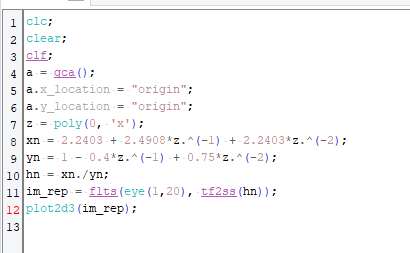
\includegraphics{code.png}	\\
	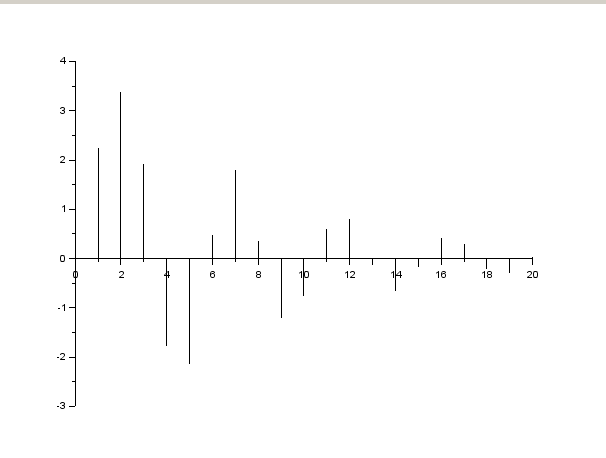
\includegraphics{graph.png}
	
\end{document}